\chapter{SYSTEM TESTING}

With the completion of system implementation, our focus now shifts towards ensuring the robustness and functionality of the system through testing. This section presents the systematic approach taken for system testing, including end-to-end testing and API testing, to validate the functionality and performance of the implemented system

\section{End-to-End Testing}

End-to-end testing is a software testing method that validates the system as a whole, ensuring that all components work together as expected. This type of testing is essential to ensure that the system meets the requirements and performs as intended. In this section, we present the end-to-end testing process for the implemented system.

\subsection{Automation tool - Cypress}

To automate the end-to-end testing process, we choose Cypress, which is a modern JavaScript-based end-to-end testing framework designed for web applications. It provides a fast, reliable, and easy-to-use testing solution for developers and QA engineers. Cypress comes with a rich set of features such as real-time reloading, automatic waiting, and built-in assertions,  allowing for efficient and effective testing of web applications.

\begin{figure}[H]
    \centering
    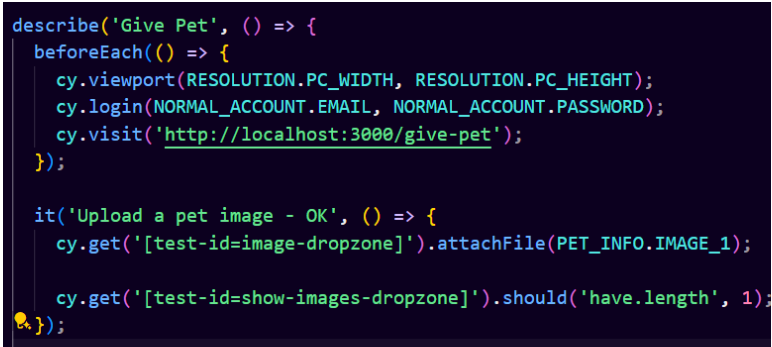
\includegraphics[width=0.7\textwidth]{Figures/cypress_script.png}
    \caption{Automation Script}
    \label{fig:cypress-script}
\end{figure}

\begin{figure}[H]
    \centering
    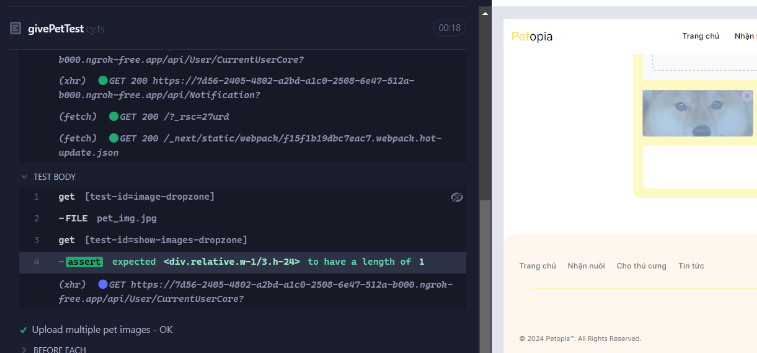
\includegraphics[width=0.7\textwidth]{Figures/cypress_auto.png}
    \caption{Automation tests done by Cypress}
    \label{fig:cypress-test}
\end{figure}

\subsection{Test Cases}
With Cypress, we tested our system features to make sure the system ran as expected and satisfied requirements. Below are some test cases of the key features and test data for them, these test cases were tested on multiple browser and environments.

\subsubsection*{Test data}

Normal User account:

\quad Email: vejox62251@facais.com - Password: 123456789

Organization User account:

\quad Email:  jayoki3306@facais.com - Password: 123456789

Owned-pet-id: baf3745f-d0d7-40c7-8084-5b55cb2f2ce3

\subsubsection*{Authentication}

\begin{longtblr}[
    caption = {Non-restricted Page Accessibility Test},
    label = {tblr:non_restricted_page_accessibility},
  ]{
    vline{1-3} = {-}{},
    hline{-} = {1-2}{},
    colspec={X[2,l] X[5, l]},
  }
  \textbf{Description} & \textbf{Non-restricted page accessibility} \\
  \textbf{Purpose} & {
    Test whether the guest user can access the pages that do not require authentication.
  } \\
  \textbf{Precondition} & {

  } \\
  \textbf{Steps} & {
    1. Click the “Nhận nuôi” button on the Nav bar.
    \\2. System shows the page content.
    \\3. Click the first pet card on the pet list.
    \\4. System shows the page content.
    \\5. Click the “Tin tức” button on the Nav bar.
    \\6. System shows the page content.
    \\7. Click the first blog card on the blog list.
    \\8. System shows the page content.
  } \\
  \textbf{Expected result} & {
    System does not direct the user to the login page.
  } \\
  \textbf{Execution results} & {
    PASSED
  } \\
\end{longtblr}




\begin{longtblr}[
    caption = {Restricted Page Accessibility Test},
    label = {tblr:restricted_page_accessibility},
  ]{
    vline{1-3} = {-}{},
    hline{-} = {1-2}{},
    colspec={X[2,l] X[5,l]},
  }
  \textbf{Description} & \textbf{Restricted page accessibility} \\
  \textbf{Purpose} & {
    Test whether the guest user can access the pages that do require authentication.
  } \\
  \textbf{Pre-condition} & {

  } \\
  \textbf{Steps} & {
    1. Click the “Cho thú cưng” button on the Nav bar.
  } \\
  \textbf{Expected result} & {
    System directs the user to the login page.
  } \\
  \textbf{Execution results} & {
    PASSED
  } \\
\end{longtblr}


\begin{longtblr}[
    caption = {Normal Account Accessibility Test},
    label = {tblr:normal_account_accessibility},
  ]{
    vline{1-3} = {-}{},
    hline{-} = {1-2}{},
    colspec={X[2,l] X[5,l]},
  }
  \textbf{Description} & \textbf{Normal account accessibility} \\
  \textbf{Purpose} & {
    Test whether the authenticated user with a normal account can access the pages that require authentication at the normal account level.
  } \\
  \textbf{Precondition} & {
    User logged in using a normal account.
  } \\
  \textbf{Steps} & {
    1. Click the “Cho thú cưng” button on the Nav bar.
  } \\
  \textbf{Expected result} & {
    System shows the restricted page content to the authenticated user.
  } \\
  \textbf{Execution results} & {
    PASSED
  } \\
\end{longtblr}


\begin{longtblr}[
    caption = {Organization Account Accessibility Test},
    label = {tblr:organization_account_accessibility},
  ]{
    vline{1-3} = {-}{},
    hline{-} = {1-2}{},
    colspec={X[2,l] X[5,l]},
  }
  \textbf{Description} & \textbf{Organization account accessibility} \\
  \textbf{Purpose} & {
    Test whether the authenticated user with an organization account can access the pages that require authentication at the organization account level.
  } \\
  \textbf{Precondition} & {
    User logged in using an organization account.
  } \\
  \textbf{Steps} & {
    1. Click the User avatar at top right.
    \\2. Click the User profile option.
    \\3. System directs to User profile page.
  } \\
  \textbf{Expected result} & {
    System shows the profile of the organization with the create blog option.
  } \\
  \textbf{Execution results} & {
    PASSED
  } \\
\end{longtblr}



\subsubsection*{Filter pet}

\begin{longtblr}[
    caption = {Filter Pets by Species Test},
    label = {tblr:filter_pets_by_species},
  ]{
    vline{1-3} = {-}{},
    hline{-} = {1-2}{},
    colspec={X[2,l] X[5,l]},
  }
  \textbf{Description} & \textbf{Filter pets by species} \\
  \textbf{Purpose} & {
    Test whether the pet list will be filtered by species.
  } \\
  \textbf{Precondition} & {
    User at search pet page.
  } \\
  \textbf{Steps} & {
    1. Click “Loài” button at the filter bar.
    \\2. Click option “Chó”.
  } \\
  \textbf{Expected result} & {
    System shows the list of dogs.
  } \\
  \textbf{Execution results} & {
    PASSED
  } \\
\end{longtblr}


The same test was done with other options: breed, age, color, sex, size, vaccinated, and spayed; which also yielded the same results. But there is a special case where breeds should be displayed according to the chosen species, so it is a separate case.

\begin{longtblr}[
    caption = {Breed Options Display According to Species Test},
    label = {tblr:breed_options_display},
  ]{
    vline{1-3} = {-}{},
    hline{-} = {1-2}{},
    colspec={X[2,l] X[5,l]},
  }
  \textbf{Description} & \textbf{Breed options display according to species} \\
  \textbf{Purpose} & {
    Test whether the breed options are displayed according to the chosen species.
  } \\
  \textbf{Precondition} & {
    User at search pet page.
  } \\
  \textbf{Steps} & {
    1. Click “Loài” button at the filter bar.
    \\2. Click option “Chó”.
    \\3. Click “Giống” button at the filter bar.
  } \\
  \textbf{Expected result} & {
    System shows a list of breeds of dogs available on the website.
  } \\
  \textbf{Execution results} & {
    PASSED
  } \\
\end{longtblr}


\subsubsection*{Account Configuration}

\begin{longtblr}[
    caption = {Update User Information Test},
    label = {tblr:update_user_information},
  ]{
    vline{1-3} = {-}{},
    hline{-} = {1-2}{},
    colspec={X[2,l] X[5,l]},
  }
  \textbf{Description} & \textbf{Update user information} \\
  \textbf{Purpose} & {
    Test whether the user can update information successfully.
  } \\
  \textbf{Precondition} & {
    User at the user profile page.
  } \\
  \textbf{Steps} & {
    1. Click the “Cập nhật thông tin” button.
    \\2. System shows the update information form.
    \\3. Fill in all the fields: First Name, Last Name, Email, Phone Number, Address.
    \\4. Click the submit button.
  } \\
  \textbf{Expected result} & {
    Account information is changed and displayed on the user profile page.
  } \\
  \textbf{Execution results} & {
    PASSED
  } \\
\end{longtblr}


\begin{longtblr}[
    caption = {Update User Information with Missing Last Name Test},
    label = {tblr:update_user_information_missing_last_name},
  ]{
    vline{1-3} = {-}{},
    hline{-} = {1-2}{},
    colspec={X[2,l] X[5,l]},
  }
  \textbf{Description} & \textbf{Update user information with missing field Last Name} \\
  \textbf{Purpose} & {
    Test whether the user can update information with a missing field.
  } \\
  \textbf{Precondition} & {
    User at the user profile page.
  } \\
  \textbf{Steps} & {
    1. Click the “Cập nhật thông tin” button.
    \\2. System shows the update information form.
    \\3. Fill in the fields: Last Name, Email, Phone Number, Address. Leave the field First Name empty.
    \\4. Click the submit button.
  } \\
  \textbf{Expected result} & {
    Submit form failed, system alerted user.
  } \\
  \textbf{Execution results} & {
    PASSED
  } \\
\end{longtblr}


The same test was done with other fields: last name, email, phone number, address; which also yielded the same results.

\subsubsection*{Give away pet}

\begin{longtblr}[
    caption = {Give Away Pet Test},
    label = {tblr:give_away_pet},
  ]{
    vline{1-3} = {-}{},
    hline{-} = {1-2}{},
    colspec={X[2,l] X[5,l]},
  }
  \textbf{Description} & \textbf{Give away pet} \\
  \textbf{Purpose} & {
    Test whether the user can give away a pet successfully.
  } \\
  \textbf{Precondition} & {
    User at the give pet page.
    \\ User is authenticated.
  } \\
  \textbf{Steps} & {
    1. System shows the give pet form. The first page is the pet image upload.
    \\2. Click the image upload zone. The system shows the upload window.
    \\3. Choose a .jpg image and click OK. The system shows the uploaded picture in the preview row.
    \\4. Click the “Tiếp tục” button. The system shows the pet information page.
    \\5. Fill in the pet information fields.
    \\6. Click the “Tiếp tục” button. The system shows pet giveaway terms.
    \\7. Tick the accept checkbox.
    \\8. Click the submit form button.
  } \\
  \textbf{Expected result} & {
    Submit pet giveaway form successfully.
  } \\
  \textbf{Execution results} & {
    PASSED
  } \\
\end{longtblr}


\begin{longtblr}[
    caption = {Submit Give Away Pet Form Without Uploading Pet Picture Test},
    label = {tblr:submit_give_away_pet_without_picture},
  ]{
    vline{1-3} = {-}{},
    hline{-} = {1-2}{},
    colspec={X[2,l] X[5,l]},
  }
  \textbf{Description} & \textbf{Submit give away pet form without uploading pet picture} \\
  \textbf{Purpose} & {
    Test whether the user can submit the give away pet form without uploading a picture of the pet.
  } \\
  \textbf{Precondition} & {
    User at the give pet page.
    \\ User is authenticated.
  } \\
  \textbf{Steps} & {
    1. System shows the give pet form. The first page is the pet image upload.
    \\2. Click the “Tiếp tục” button. System shows the pet information page.
    \\3. Fill in the pet information fields.
    \\4. Click the “Tiếp tục” button. System shows pet giveaway terms.
    \\5. Tick the accept checkbox.
    \\6. Click the submit form button.
  } \\
  \textbf{Expected result} & {
    Submit pet giveaway form fails. System alerts the user.
  } \\
  \textbf{Execution results} & {
    PASSED
  } \\
\end{longtblr}


\begin{longtblr}[
    caption = {Submit Give Away Pet Form Without Pet Information Test},
    label = {tblr:submit_give_away_pet_without_info},
  ]{
    vline{1-3} = {-}{},
    hline{-} = {1-2}{},
    colspec={X[2,l] X[5,l]},
  }
  \textbf{Description} & \textbf{Submit give away pet form without pet information} \\
  \textbf{Purpose} & {
    Test whether the user can submit the give away pet form without giving the information of the pet.
  } \\
  \textbf{Precondition} & {
    User at the give pet page.
    \\ User is authenticated.
  } \\
  \textbf{Steps} & {
    1. System shows the give pet form. The first page is the pet image upload.
    \\2. Click the image upload zone. System shows the upload window.
    \\3. Choose a .jpg image and click OK. The system shows the uploaded picture in the preview row.
    \\4. Click the “Tiếp tục” button. System shows the pet information page.
    \\5. Click the “Tiếp tục” button. System shows pet giveaway terms.
    \\6. Tick the accept checkbox.
    \\7. Click the submit form button.
  } \\
  \textbf{Expected result} & {
    Submit pet giveaway form fails. System alerts the user.
  } \\
  \textbf{Execution results} & {
    PASSED
  } \\
\end{longtblr}


\begin{longtblr}[
    caption = {Submit Give Away Pet Form Without Reading Give Away Terms Test},
    label = {tblr:submit_give_away_pet_without_terms},
  ]{
    vline{1-3} = {-}{},
    hline{-} = {1-2}{},
    colspec={X[2,l] X[5,l]},
  }
  \textbf{Description} & \textbf{Submit give away pet form without reading give away terms} \\
  \textbf{Purpose} & {
    Test whether the user can submit the give away pet form without reading the terms.
  } \\
  \textbf{Precondition} & {
    User at the give pet page.
    \\ User is authenticated.
  } \\
  \textbf{Steps} & {
    1. System shows the give pet form. The first page is the pet image upload.
    \\2. Click the “Tiếp tục” button. System shows the pet information page.
    \\3. Click the “Tiếp tục” button. System shows pet giveaway terms.
    \\4. Try to tick the accept checkbox.
  } \\
  \textbf{Expected result} & {
    Cannot tick the accept checkbox. System alerts the user.
  } \\
  \textbf{Execution results} & {
    PASSED
  } \\
\end{longtblr}


\subsubsection*{Adopt Pet}

\begin{longtblr}[
    caption = {Adopt Pet Test},
    label = {tblr:adopt_pet},
  ]{
    vline{1-3} = {-}{},
    hline{-} = {1-2}{},
    colspec={X[2,l] X[5,l]},
  }
  \textbf{Description} & \textbf{Adopt pet} \\
  \textbf{Purpose} & {
    Test whether the user can submit an adopt application successfully.
  } \\
  \textbf{Precondition} & {
    User at the search pet page.
    \\ User is authenticated.
  } \\
  \textbf{Steps} & {
    1. Click the first pet card on the pet list.
    \\2. System directs to the pet detail page.
    \\3. Click the “Nhận nuôi” button.
    \\4. System shows the adopt application form.
    \\5. Fill in all required information: name, email, phone number, address, home type, adopt time, note, pets owned.
    \\6. Click the submit button.
  } \\
  \textbf{Expected result} & {
    User submits adopt application successfully.
  } \\
  \textbf{Execution results} & {
    PASSED
  } \\
\end{longtblr}


\begin{longtblr}[
    caption = {Submit Adopt Pet on Already Submitted Pet Test},
    label = {tblr:submit_adopt_pet_again},
  ]{
    vline{1-3} = {-}{},
    hline{-} = {1-2}{},
    colspec={X[2,l] X[5,l]},
  }
  \textbf{Description} & \textbf{Submit adopt pet on already submitted pet} \\
  \textbf{Purpose} & {
    Test whether the user can submit an adopt application again on the same pet.
  } \\
  \textbf{Precondition} & {
    User at the search pet page.
    \\ User is authenticated.
    \\ Already done the Adopt pet test case.
  } \\
  \textbf{Steps} & {
    1. Click the first pet card on the pet list.
    \\2. System directs to the pet detail page.
    \\3. Click the “Nhận nuôi” button.
  } \\
  \textbf{Expected result} & {
    System alerts the user that they already sent the adopt application for this pet.
  } \\
  \textbf{Execution results} & {
    PASSED
  } \\
\end{longtblr}


\begin{longtblr}[
    caption = {Adopt Owned Pet Test},
    label = {tblr:adopt_owned_pet},
  ]{
    vline{1-3} = {-}{},
    hline{-} = {1-2}{},
    colspec={X[2,l] X[5,l]},
  }
  \textbf{Description} & \textbf{Adopt owned pet} \\
  \textbf{Purpose} & {
    Test whether the user can submit an adopt application for a pet that has already been adopted.
  } \\
  \textbf{Precondition} & {
    User is authenticated.
    \\ System has owned pet.
  } \\
  \textbf{Steps} & {
    1. Use the owned pet ID in the test data to visit the pet detail page by adding “/pet/[pet-id]” to the website URL.
    \\2. System directs to the pet detail page.
  } \\
  \textbf{Expected result} & {
    The “Nhận nuôi” button is not available.
  } \\
  \textbf{Execution results} & {
    PASSED
  } \\
\end{longtblr}


\subsubsection*{Blog}

\begin{longtblr}[
    caption = {Blog Browsing - Blog Card Linking Test},
    label = {tblr:blog_card_linking},
  ]{
    vline{1-3} = {-}{},
    hline{-} = {1-2}{},
    colspec={X[2,l] X[5,l]},
  }
  \textbf{Description} & \textbf{Blog browsing - Blog card linking} \\
  \textbf{Purpose} & {
    Test whether the blog card directs to the correct blog.
  } \\
  \textbf{Precondition} & {
    User at the blog page.
  } \\
  \textbf{Steps} & {
    1. Click the first blog card.
    \\2. System directs to the blog detail page.
  } \\
  \textbf{Expected result} & {
    System displays the blog detail page related to the chosen blog card.
  } \\
  \textbf{Execution results} & {
    PASSED
  } \\
\end{longtblr}


\begin{longtblr}[
    caption = {Blog Browsing - Filter Blog by Health Category Test},
    label = {tblr:filter_blog_by_health_category},
  ]{
    vline{1-3} = {-}{},
    hline{-} = {1-2}{},
    colspec={X[2,l] X[5,l]},
  }
  \textbf{Description} & \textbf{Blog browsing - Filter blog by health category} \\
  \textbf{Purpose} & {
    Test whether the blog cards will be filtered by the category bar.
  } \\
  \textbf{Precondition} & {
    User at the blog page.
  } \\
  \textbf{Steps} & {
    1. Click the “Sức khỏe” option in the category bar.
    \\2. System displays new filtered blog cards.
  } \\
  \textbf{Expected result} & {
    System only displays the blogs about health.
  } \\
  \textbf{Execution results} & {
    PASSED
  } \\
\end{longtblr}


The same test was done with other categories: art, training, and product; which also yielded the same results.

\begin{longtblr}[
    caption = {Blog Create Test},
    label = {tblr:blog_create},
  ]{
    vline{1-3} = {-}{},
    hline{-} = {1-2}{},
    colspec={X[2,l] X[5,l]},
  }
  \textbf{Description} & \textbf{Blog create} \\
  \textbf{Purpose} & {
    Test whether the user can create a blog.
  } \\
  \textbf{Precondition} & {
    User is logged in using an organization account.
    \\ User is at the user profile page.
  } \\
  \textbf{Steps} & {
    1. Click the blog tab. System displays the blog tab content.
    \\2. Click the create blog card.
    \\3. System directs to the blog create page.
    \\4. Fill in the required fields: title, excerpt, blog image, blog content.
    \\5. Click the submit button.
  } \\
  \textbf{Expected result} & {
    User creates the blog successfully.
  } \\
  \textbf{Execution results} & {
    PASSED
  } \\
\end{longtblr}


\begin{longtblr}[
    caption = {Blog Update Test},
    label = {tblr:blog_update},
  ]{
    vline{1-3} = {-}{},
    hline{-} = {1-2}{},
    colspec={X[2,l] X[5,l]},
  }
  \textbf{Description} & \textbf{Blog Update} \\
  \textbf{Purpose} & {
    Test whether the user can update a created blog.
  } \\
  \textbf{Precondition} & {
    User is logged in using an organization account.
    \\ User is at the user profile page.
    \\ Have done the previous Blog Create Test-case.
  } \\
  \textbf{Steps} & {
    1. Click the blog tab. System displays the blog tab content.
    \\2. Click the edit button on the created blog.
    \\3. System opens the blog update form.
    \\4. Change the blog title, content, excerpt, image.
    \\5. Click the submit button.
  } \\
  \textbf{Expected result} & {
    User updates the blog successfully.
  } \\
  \textbf{Execution results} & {
    PASSED
  } \\
\end{longtblr}


\section{API Testing}

